% Copyright 2004 by Till Tantau <tantau@users.sourceforge.net>.
%
% In principle, this file can be redistributed and/or modified under
% the terms of the GNU Public License, version 2.
%
% However, this file is supposed to be a template to be modified
% for your own needs. For this reason, if you use this file as a
% template and not specifically distribute it as part of a another
% package/program, I grant the extra permission to freely copy and
% modify this file as you see fit and even to delete this copyright
% notice. 
\def\ACCOMPLETE{}
\documentclass{beamer}
\usepackage{color}
\usepackage{graphicx}
\usepackage{marvosym}
\usepackage{tikz}
\setbeamertemplate{items}[circle]
\setbeamercovered{transparent}

\usetheme{Madrid}
\newcommand{\mc}{\mathcal}
\newcommand{\mb}{\mathbf}
\newcommand{\tr}{\text{Tr}}
\newcommand\numberthis{\addtocounter{equation}{1}\tag{\theequation}}
\let\oldnl\nl
\newcommand{\nonl}{\renewcommand{\nl}{\let\nl\oldnl}}

\DeclareMathOperator*{\argmin}{arg\,min}
\DeclareMathOperator*{\vcdim}{VC-Dim}

\newcommand\mynum[1]{%
  \usebeamercolor{enumerate item}%
  \tikzset{beameritem/.style={circle,inner sep=0,minimum size=2ex,text=enumerate item.bg,fill=enumerate item.fg,font=\footnotesize}}%
  \tikz[baseline=(n.base)]\node(n)[beameritem]{#1};%
}

\title[Efficient Clustering]{Theoretical foundations for efficient clustering}

\author[S. Kushagra]{
Shrinu Kushagra\\
\vspace{30pt}Ph.D Thesis Presentation\\
University of Waterloo
}
\date{\today}

\AtBeginSubsection[]
{
  \begin{frame}<beamer>
  \frametitle{Outline}
    \tableofcontents[currentsection]
  \end{frame}
}

% Let's get started
\begin{document}

\begin{frame}
  \titlepage
\end{frame}

\begin{frame}{What is clustering?}
	Given: $X$\\
	\vspace{10pt}Partition it into $k$ subsets .$$C = \{C_1, \ldots, C_k\}$$
	\begin{itemize}
		\item Similar points share a cluster.
		\item Dis-similar points are separated.
	\end{itemize}
\end{frame}

\begin{frame}<1>[label=clusteringChallenges]{Challenges in clustering}
	\begin{enumerate}
		\onslide<1> \item Computational complexity
		\onslide<2> \vspace{20pt}\item  Under-specificity
		\onslide<3>\vspace{20pt}\item Noise robustness
	\end{enumerate}
\end{frame}

\begin{frame}{Computational cost}
	Common approach to clustering
	\begin{itemize}
		\item Associate cost with each partition of the set.
		\item Find partition with minimum cost.
	\end{itemize}

	\vspace{20pt}$k$-means is NP-Hard.
	\begin{itemize}
		\item NP-Hard for $k=2$ \alert{[Dasgupta `08]}
		\vspace{0pt}\item NP-Hard in the plane. \alert{[Vattani `09]}
		\vspace{0pt}\item NP-Hard to approximate within $(1+\epsilon)$ \alert{[Awasthi et. al `15]}
	\end{itemize} 
	
	\vspace{20pt}$k$-median is NP-Hard \alert{[Megiddo, Supowit `84]}.
	\begin{itemize}
		\vspace{0pt}\item $(3+\epsilon)$-approximation is known. \alert{[Arya et. al `04]}
	\end{itemize}		
\end{frame}

\begin{frame}<2>[label=clusteringChallenges]{Challenges in clustering}
	\begin{enumerate}
		\onslide<1> \item Computational complexity
		\onslide<2> \vspace{20pt}\item  Under-specificity
		\onslide<3>\vspace{20pt}\item Noise robustness
	\end{enumerate}
\end{frame}

\begin{frame}{Under-specificity in clustering}
	
	Requirements from clustering algorithms\\
	\vspace{10pt}
	\begin{block}{}
		\begin{itemize}
			\item Similar points together
			\item Dis-similar points separated
		\end{itemize}
	\end{block}
	
	\vspace{10pt}\alert{Conflicting}
	\begin{center}
	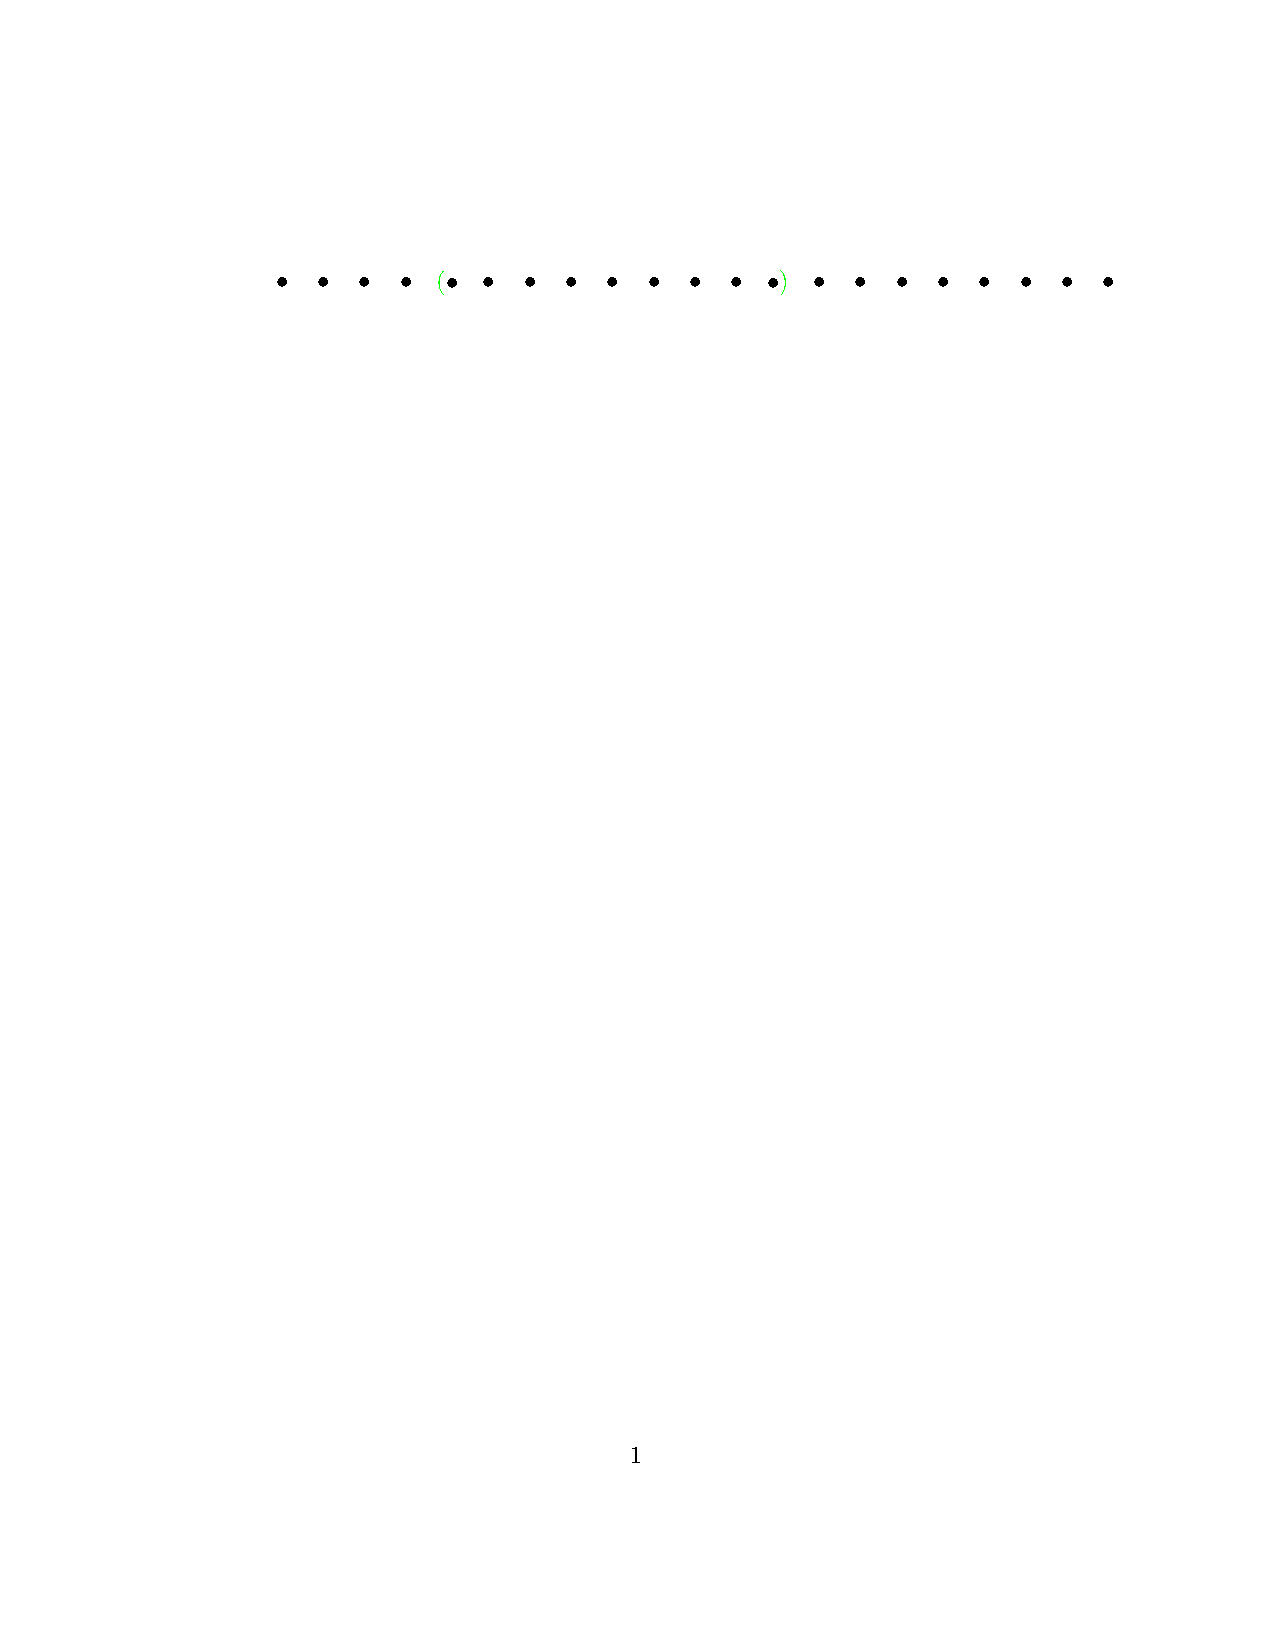
\includegraphics[trim={100 650 30 120},clip,width=0.8\textwidth]{figures/conflictingReq.pdf}
	\end{center}
\end{frame}

\begin{frame}{Example}
	Given $X \in \mb R^2$ and $k = 2$
	\begin{center}
	\begin{figure}
	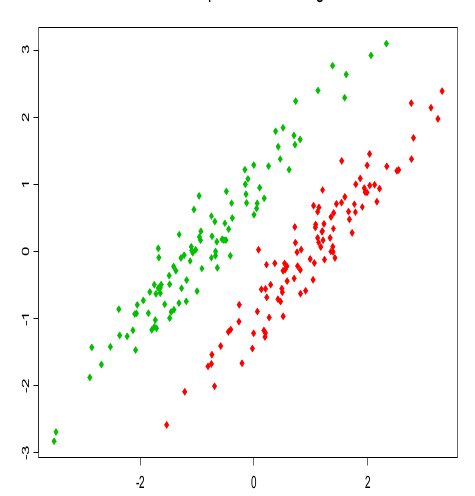
\includegraphics[trim={0 0 0 20},clip,width=0.4\textwidth]{figures/slX.png}
	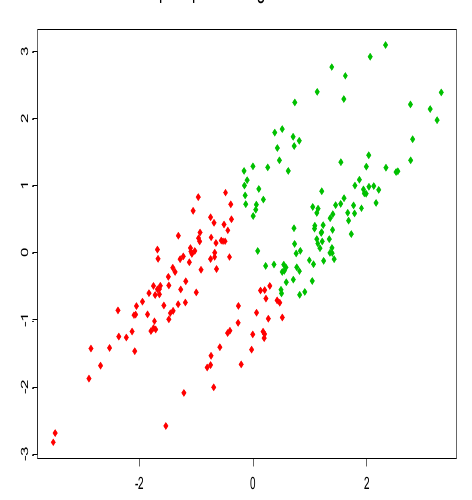
\includegraphics[trim={0 0 0 20},clip,width=0.4\textwidth]{figures/kmeansX.png}
	\caption{Single-linkage on our example dataset (Left). $k$-means on our example dataset (Right)}
	\end{figure}
	\end{center}
\end{frame}

\begin{frame}{Different algorithms have different considerations}
	
	Single-linkage\\
	\begin{itemize}
		\item Similar points together, dis-similar can end up together.
	\end{itemize}
	
	\vspace{10pt}$k$-means\\
	\begin{itemize}
		\item Separate dissimilar points, similar can be separated. 
	\end{itemize}
	
	 \vspace{20pt}\alert{Model selection problem:} How to prefer one choice over the other?
\end{frame}

\begin{frame}<3>[label=clusteringChallenges]{Challenges in clustering}
	\begin{enumerate}
		\onslide<1> \item Computational complexity
		\onslide<2> \vspace{20pt}\item  Under-specificity
		\onslide<3>\vspace{20pt}\item Noise robustness
	\end{enumerate}
\end{frame}

\begin{frame}{Noise-robustness}
	
	Clustering definition revisited.
	\begin{block}{}
		\begin{itemize}
			\item Similar points together
			\item Dis-similar points separated
		\end{itemize}
	\end{block}
	
	\vspace{30pt}Makes sense when data has cohesive structure.
	\begin{itemize}
		\vspace{10pt}\item Subsets which are \textcolor{blue}{well-separated}.
	\end{itemize}
\end{frame}

\begin{frame}{Noise-robustness}
	Real world data
	\begin{itemize}
		\vspace{10pt}\item Well-clustered subset
		\vspace{5pt}\item Unstructured part
	\end{itemize}
	
	\vspace{25pt}How to detect structure in the presence of noise?
\end{frame}

\begin{frame}{Summary: Challenges in clustering}
	\begin{enumerate}
		\item Computational complexity
		\vspace{20pt}\item  Under-specificity
		\vspace{20pt}\item Noise robustness
	\end{enumerate}
\end{frame}

\begin{frame}<1>{Outline}
	First part
	\vspace{10pt}\begin{block}{}
	\mynum{2} Under-specificity \alert{and} \\\vspace{10pt}\mynum{1} Computational complexity
	\end{block}
		
	\onslide<2>\vspace{35pt}Second part
	\vspace{10pt}\begin{block}{}
	\mynum{3} Noise-robustness \alert{and} \\\vspace{10pt}\mynum{1} Computational complexity
	\end{block}		
\end{frame}

\begin{frame}{Dealing with under-specificity}

	Incorporating domain knowledge into the clustering problem\\	
	\begin{itemize}
		\vspace{10pt} \item Must/cannot link constraints \alert{[Basu et. al `02]}\\
		\vspace{10pt} \item Demonstration-based clustering \alert{[Ashtiani, Ben-David `15]}\\
		\vspace{10pt} \item Merge/split queries \alert{[Balcan, Blum `08]}
	\end{itemize}
\end{frame}

\begin{frame}{Our approach}
	
	{\color{blue}Same-cluster query}\\
    \vspace{20pt}Given a clustering $C^*$ of set $X$\\
    \vspace{5pt}Ask same-cluster queries to a $C^*$-oracle\\
    $$C^*(x_1, x_2) = \left\{
	\begin{array}{ll}
		\mbox{true }  & \mbox{if } x_1 \overset{C^*}{\sim} x_2   \\
		\mbox{false } & otherwise 
	\end{array}
\right. $$
\end{frame}

\begin{frame}{Center-based clustering with same-cluster queries}
	\begin{itemize}
		\item Joint work with Hassan Ashtiani and Shai Ben-David
		\vspace{20pt} \item In proceedings of \alert{NeurIPS'16}.
	\end{itemize}
\end{frame}

\begin{frame}{Problem Setting}
	Input: $X \subseteq \mb R^d$
	\begin{itemize} 
   		\vspace{10pt}\item Learner can make same-cluster queries to $C^*$-oracle
		\vspace{10pt}\item Oracle's clustering is ``nice".     
	\end{itemize}
	\vspace{20pt} {\color{blue}Goal}: Recover the oracle's clustering $C^* = \{C_1^*, \ldots, C_k^*\}$
\end{frame}

\begin{frame}{$\gamma$-margin niceness}
	Cluster-center is closer to its own points than to points outside.
	\vspace{1cm}\begin{figure}        
            \centering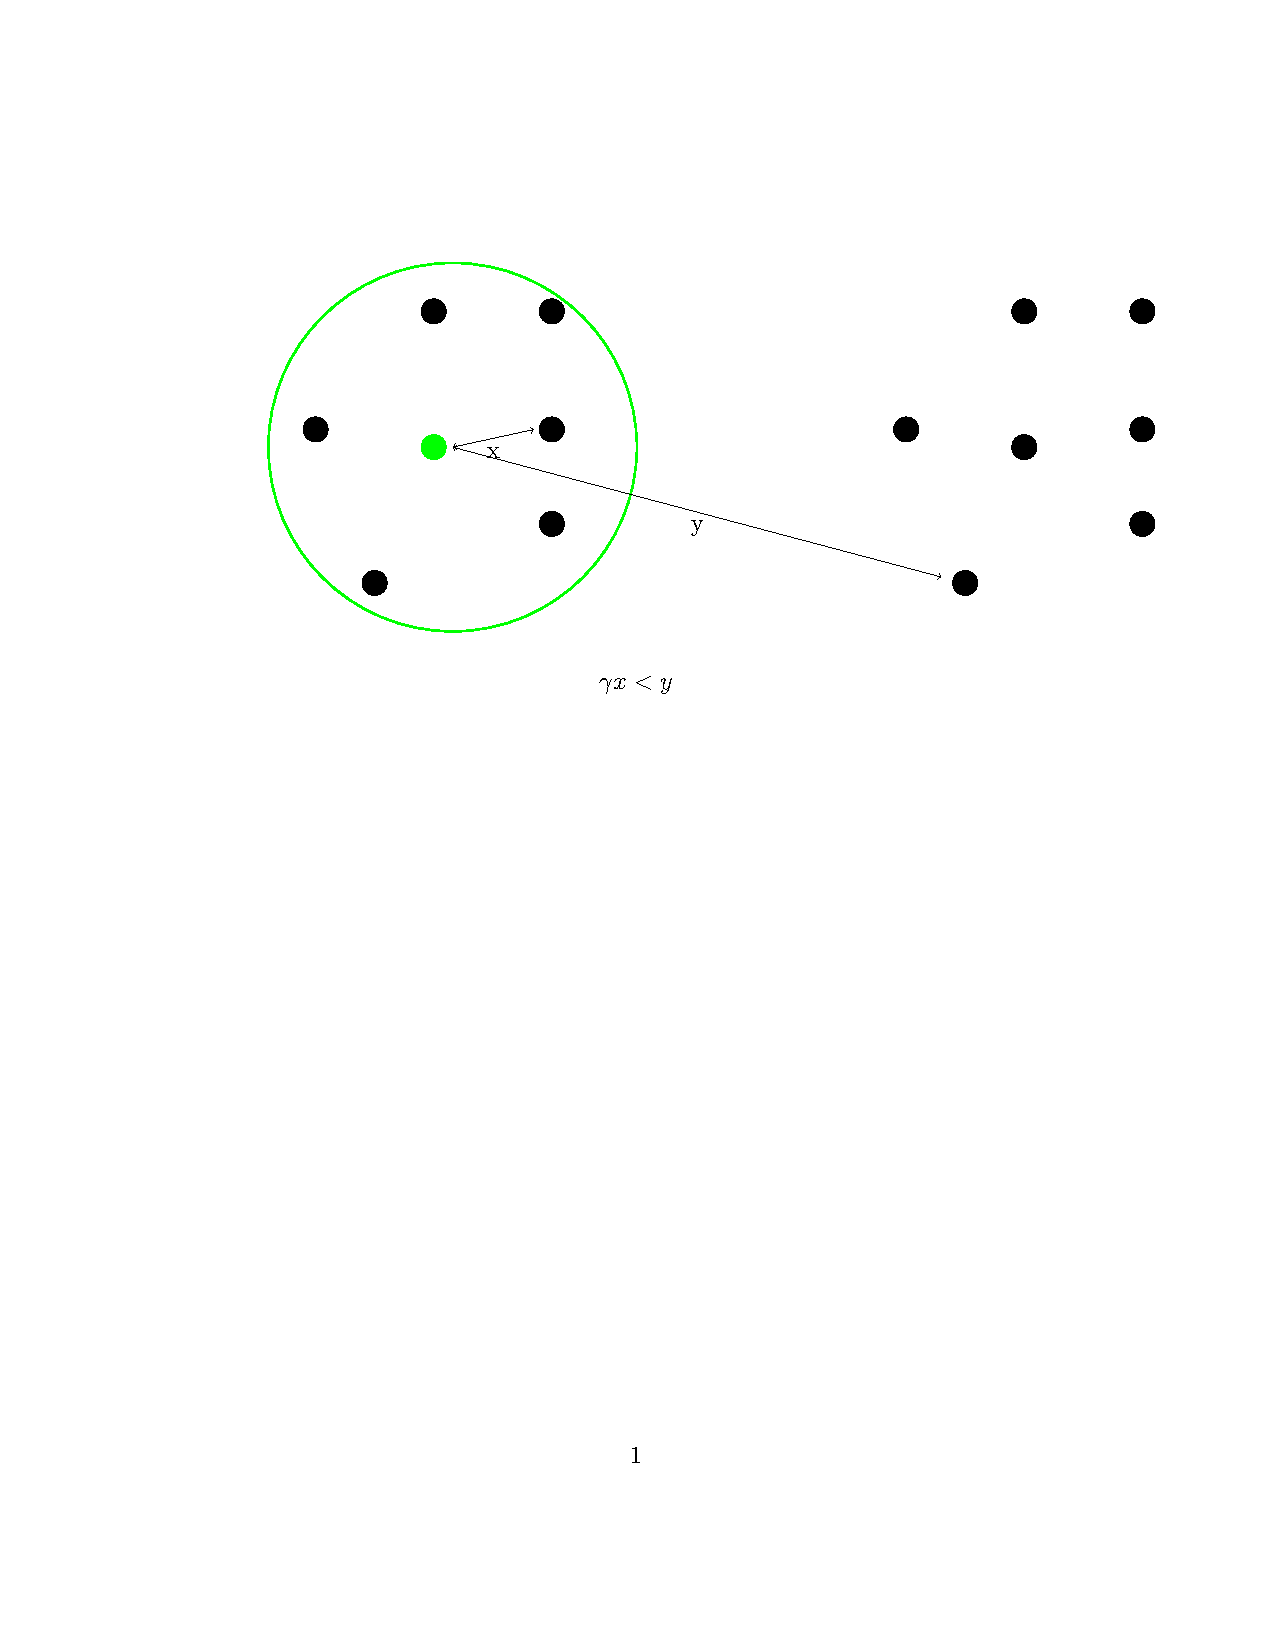
\includegraphics[trim= 400 470 400 150, scale=0.5]{figures/gammaMargin.pdf}
    \end{figure} 
    \begin{block}{}
		For all $i$, for all $x \in C_i$ and for all $y \not\in C_i$
		$$\gamma d(x, \mu_i) < d(y, \mu_i)$$	
	\end{block}  
\end{frame}

\begin{frame}{Sidenote: Results under margin assumption (no queries)}
  Given: $X$ and $k$\\
  \vspace{10pt}Optimal solution to the desired objective function satisfies $\gamma$-margin.

	\vspace{20pt}\begin{table}[]
	\centering
	%\caption{My caption}
	\label{my-label}
	\begin{tabular}{lll|lll|}
	& $k$-means &  &  &    & \begin{tabular}[c]{@{}l@{}}Poly-time solvable for $\gamma \ge 3$\\ NP-Hard for $\gamma < 3$\end{tabular} \\\\
	\hline\\
	& $k$-median &  &  &  & \begin{tabular}[c]{@{}l@{}}Poly-time solvable for $\gamma \ge 2$\\ NP-Hard for $\gamma < 2$\end{tabular}
	\end{tabular}
	\end{table}
\end{frame}

\begin{frame}{Problem Setting}
	Input: $X \subseteq R^d$
	\begin{itemize} 
   		\vspace{10pt}\item Learner can make same-cluster queries to $C^*$-oracle
		\vspace{10pt}\item $C^*$ satisfies $\gamma$-margin
		\vspace{10pt}\item $\mu_i^*$ is  the center of mass of $C_i^*$
	\end{itemize}
	\vspace{20pt} {\color{blue}Goal}: Recover the oracle's clustering $C^* = \{C_1^*, \ldots, C_k^*\}$
\end{frame}

\begin{frame}{Clustering with queries}
  \begin{block}{The algorithm}
	\vspace{10pt}
	1. Estimate center
	\begin{itemize}
		\item Query uniformly till we have ``enough'' points from one cluster
    \end{itemize}  
	\vspace{10pt}
	2. Compute radius
	\begin{itemize}
	  \item Binary search to find the ``radius"
    \end{itemize}  
	\vspace{10pt}
	3. Delete and repeat
  \end{block}
\end{frame}

\begin{frame}{Results}

	\begin{block}{Positive result with queries}
		\vspace{10pt}For $\gamma > 1$, our algorithm finds $C^*$ (with high probability) and 
		\begin{itemize}
		\vspace{10pt}\item Runs in $O(kn\log n)$ time.
        \vspace{10pt}\item Makes $O(k^2\log k + k\log n)$ same-cluster queries.
		\end{itemize}
	\end{block}
	
	\vspace{20pt}Query complexity: Logarithmic\\
	\vspace{10pt}Any target clustering $C^*$ as long the niceness conditions are satisfied. 
\end{frame}

\begin{frame}{$k$-means revisited}
	\vspace{-20pt}Input: $X \subseteq \mb R^d$ and $k$.
	\vspace{-10pt}$$C^* = \argmin_{C} \sum_{i=1}^k \sum_{x \in C_i} \|x - \mu_i\|^2$$
	\vspace{10pt}Given that $C^*$ satisfies $\gamma$-margin\\
	
	\vspace{10pt}\begin{block}{Theorem}
	Euclidean $k$-means is NP-hard even when the optimal solution satisfies the $\gamma$-margin property for $\gamma < 1.84$
	\end{block}
	
	\vspace{20pt} Can efficiently find the optimal using $O(k\log n)$ queries for $\gamma > 1$
\end{frame}

\begin{frame}{Hardness result}
	\begin{itemize}
		\item Reduction from exact cover by $3$-sets ($X3C$)
		\item Hard for $k = \Theta(n^\epsilon)$ and $d = 2$.
		\item Similar ideas as in \alert{[Vattani'09]}
	\end{itemize}
	
	\begin{figure}
		\centering
		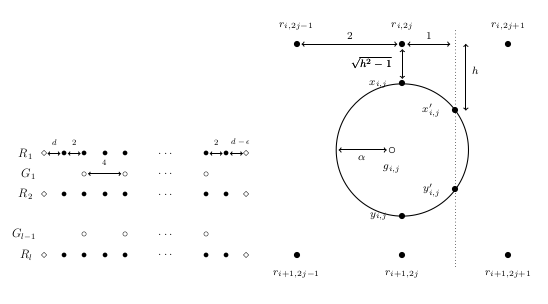
\includegraphics[trim=0 0 0 0,scale=0.5]{figures/hardnessFig.png}
	\end{figure}
\end{frame}

\begin{frame}{Key Takeaways}
	
	\begin{itemize}
		\item Same-cluster queries tackle under-specificity.
		\vspace{30pt}\item NP-Hard problem becomes {\color{blue}tractable with few queries}. 
	\end{itemize}
\end{frame}


\begin{frame}{Data de-duplication with same-cluster queries}
	\begin{itemize}
		\item Joint work with Shai Ben-David and Ihab Ilyas.
		\vspace{20pt}\item Experiments and hashing based algorithms are joint work with Hemant Saxena.		
		\vspace{20pt} \item In proceedings of \alert{AISTATS'19} and \alert{ICDE'19}.
	\end{itemize}
\end{frame}

\begin{frame}{De-duplication}
	\onslide<1->
    Given a database $X$. \\
    \vspace{10pt}Detect records which correspond to the same real-world entity.
    
    \vspace{30pt}Output a clustering of $X$.
    $$C = \{C_1, \ldots, C_k \}$$
    where $C_i \cap C_j = \phi$ and $\cup C_i = X$.
\end{frame}

\begin{frame}{Clustering for de-duplication}
	Challenges\\
    \begin{itemize}
    	\vspace{20pt}\item Standard techniques like $k$-means, $k$-median etc. are not suitable.\\
    	\textcolor{blue}{$k$ is unknown.}
	\end{itemize}    	
\end{frame}

\begin{frame}{Correlation clustering (CC) for de-duplication}
	Input: $X$\\
	Metric: $d$ over $X^2$\\
	\begin{itemize}
		\item User designed (prior knowledge of domain) 
		\item Learned from labelled data.
	\end{itemize}
	 
	\vspace{20pt}Graph $G = (X, E)$. \\
    \vspace{10pt}Find a clustering which minimizes
    
    \begin{center}
    \textcolor{blue}{\# zero edges within a cluster + \# one edges\\ across different clusters}
    \end{center}
    
\end{frame}

\begin{frame}{CC framework: Missing pieces}
	Agnostic to some information ``stored" in the metric $d$ (or the edges $E$)
    \begin{itemize}
    	\vspace{10pt}\item If $E$ corresponds to a clustering, then finding that clustering is easy.\\
    	\vspace{10pt}\item What if the optimal solution is `close to' $E$ ? 
	\end{itemize}
	
	\onslide<2->
	\vspace{20pt}Applicability of human supervision
	\begin{itemize}
    	\vspace{10pt}\item Given two records $r_1$ and $r_2$, do they correspond to the same or different real-world entity?.
	\end{itemize}
\end{frame}

\begin{frame}{Promise Correlation Clustering (PCC)}
	\begin{block}{Input}
		$G = (X, E)$
	\end{block}
	
	\begin{block}{Find}
	\vspace{-15pt}\begin{align*}
	  &C^* = \argmin_{C \in \mc F} \enspace \text{correlation-loss}_{E}(C) \label{eqn:promiseCorrLoss}
	\end{align*}
	
	\vspace{-10pt}\begin{itemize}
		\item $\mc F$ is the set of all possible clusterings $C$ such that $m(C) \le M$.
		\item $E$ is $(\alpha, \beta)$-informative
	\end{itemize}		
	\end{block}
	
	\begin{block}{$(\alpha, \beta)$-informative}
		
		\vspace{-10pt}\begin{align*}
			&\underset{(x, y) \sim U^2}{\mb P}\enspace \big[ d(x, y) > \lambda \enspace|\enspace C^*(x, y) = 1\big] \enspace \le \enspace \alpha \\
			&\underset{(x, y) \sim U^2}{\mb P}\enspace \big[C^*(x, y) = 1 \enspace|\enspace d(x, y) \le \lambda \big] \enspace \ge \enspace \beta 
		\end{align*}
	\end{block}	
\end{frame}

\begin{frame}{Goals}

	\begin{itemize}
		\item Analyse the computation complexity of PCC.
		\vspace{30pt}\item In the presence of oracle, also analyse the query complexity.
	\end{itemize}	 
\end{frame}

\begin{frame}{PCC is NP-Hard}
	\begin{block}{Theorem}
		Finding the optimal solution to the Promise Correlation Clustering problem is NP-Hard for all $M \ge 3$ and for $\alpha = 0$ and $\beta = \frac{1}{2}$.  
	\end{block}
	
	\onslide<2->
	\vspace{20pt}
	\begin{itemize}
		\item Reduction from Exact Cover by $3$-sets (X3C).\\
		\vspace{10pt}\item Similar gadget as reduction of X3C to Partition into Triangles (PIT) problem.
		\vspace{10pt}\item Using an optimization algorithm to solve the decision problem.  

	\end{itemize}
\end{frame}

\begin{frame}{Hardness of PCC}
	\begin{columns}
		\begin{column}{0.48\textwidth}
			\vspace{-40pt}\begin{figure}
				\centering
				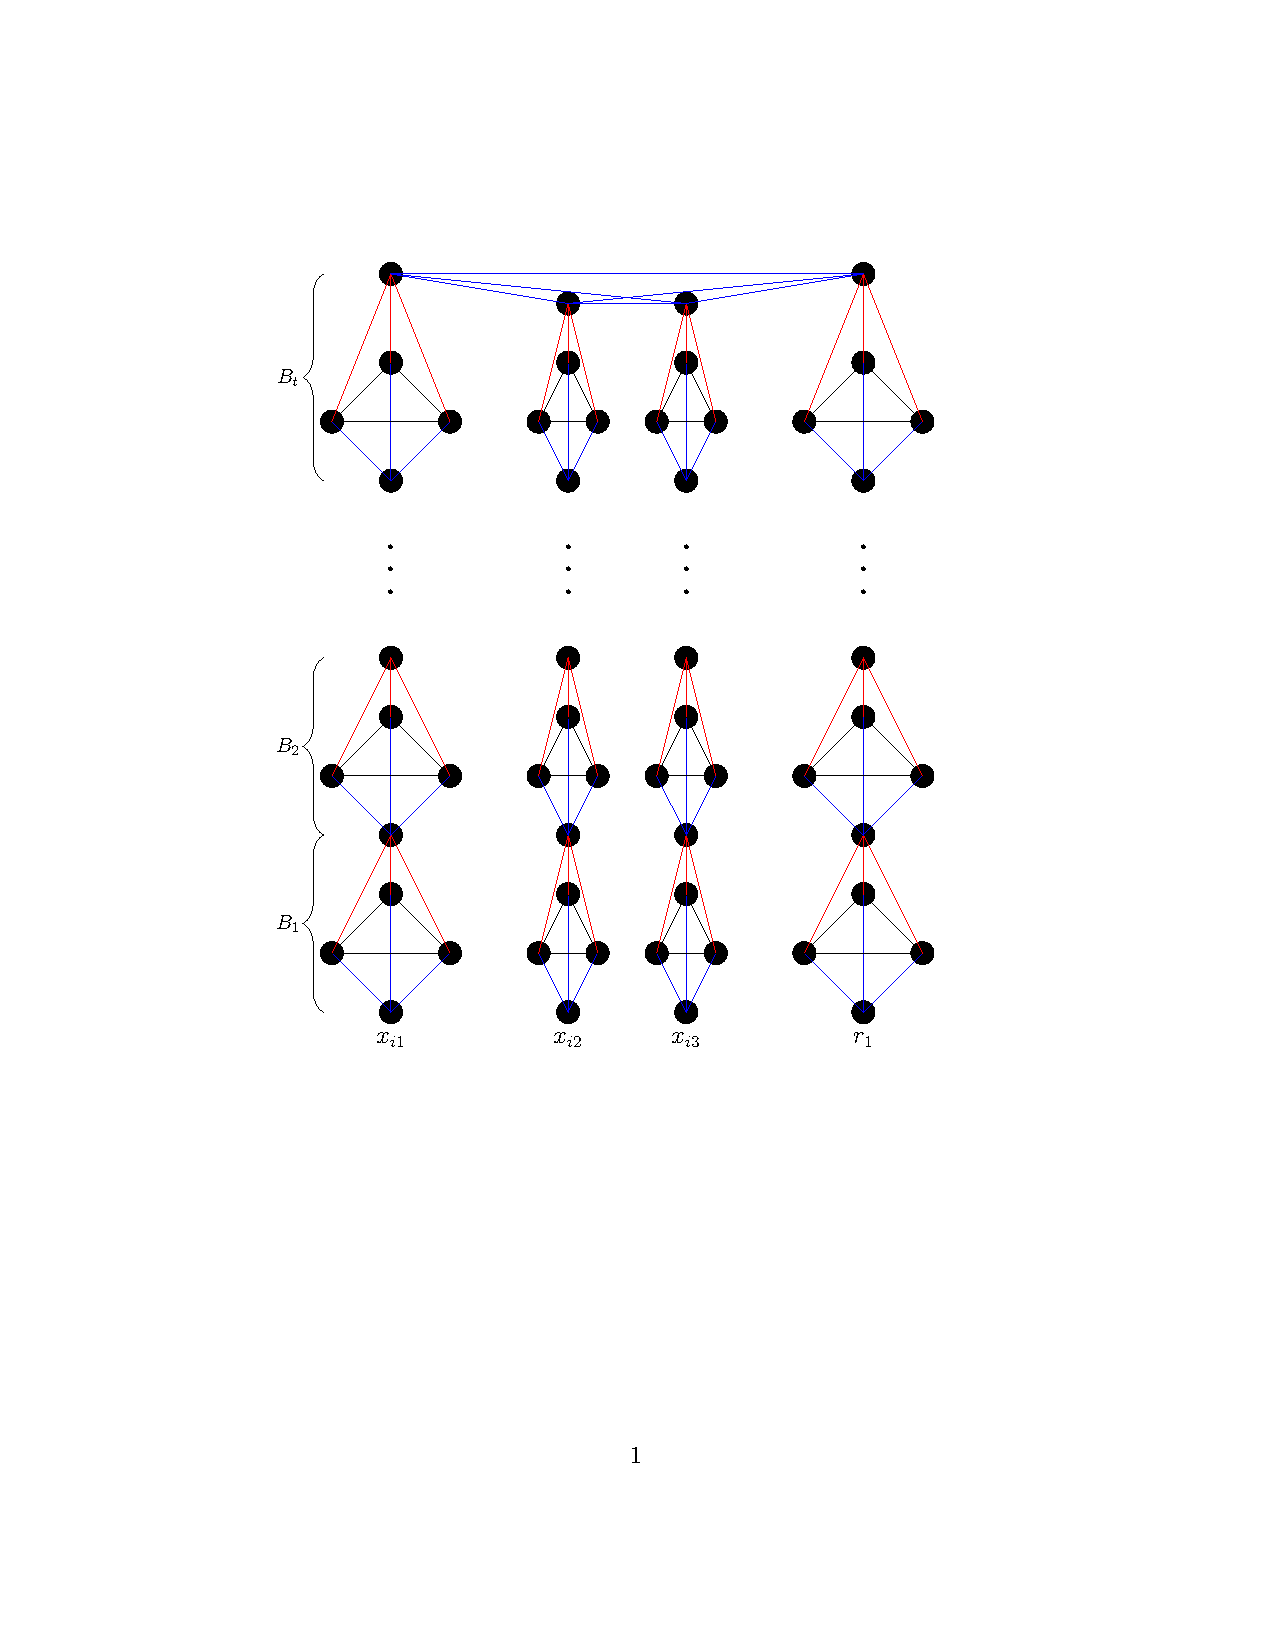
\includegraphics[trim = 100 290 100 100, clip, width=6cm, height=4.5cm]{figures/deDuplication/pccHard.pdf}
			\end{figure}
		\end{column}

		\begin{column}{0.48\textwidth}
		    Part of graph $G$ constructed by local replacement for the subset $S_i =  \{x_{i1}, x_{i2}, x_{i3}\}$. Illustration for $M = 4$.
		\end{column}
	\end{columns}

	
	\vspace{20pt}\begin{itemize}
		\item If $A$ outputs a clustering such that all clusters have size $M$ and no negative erros, then output YES.
		\vspace{10pt}\item Else NO.
	\end{itemize}
\end{frame}

\begin{frame}{Goals}
	Analyse the computation complexity of PCC.
	\begin{itemize}
		\vspace{10pt}\item NP-Hard.
	\end{itemize}	 
	\vspace{30pt}Analyse the computation complexity of PCC in the presence of an oracle.
	\begin{itemize}
		\vspace{10pt}\item Easy with $|X|^2$ queries.
		\vspace{10pt}\item If $\alpha = 0$ then easy with $O(\beta|X|)$ queries.
	\end{itemize}
\end{frame}

\begin{frame}{Hardness of PCC in the presence of an oracle}
	\begin{block}{Theorem}
		Given that the Exponential Time Hypothesis (ETH) holds. Any algorithm for PCC that runs in polynomial time makes $\Omega(|X|)$ same-cluster queries for all $M \ge 3$ and for $\alpha = 0$ and $\beta = \frac{1}{2}$. 
	\end{block}
	\onslide<2->
	\vspace{20pt}Strategy: Any algorithm for PCC takes $2^{\Omega(n)}$ time.
	\begin{itemize}
		\vspace{10pt}\item Any algorithm for X3C or equivalently 3DM takes $2^{\Omega(m)}$ time.
	\end{itemize}
\end{frame}

\begin{frame}{3SAT to 3DM}
	Classical constructions are `inefficient'.\\
	\begin{itemize}
	\vspace{10pt}\item \alert{[Johnson and Garey'79]} proof translates to $2^{\Omega(m^{0.25})}$ lower bound for 3DM.
	\end{itemize}
	\vspace{20pt}Ideas similar to \alert{[Charikar, Guruswami, Wirth'04]}.\\
	\vspace{20pt}Linear reduction of independent interest.	
\end{frame}

\begin{frame}{Hardness: Linear reduction of 3SAT to 3DM}
	\begin{columns}
		\begin{column}{0.48\textwidth}
			\vspace{-40pt}\begin{figure}
				\centering
				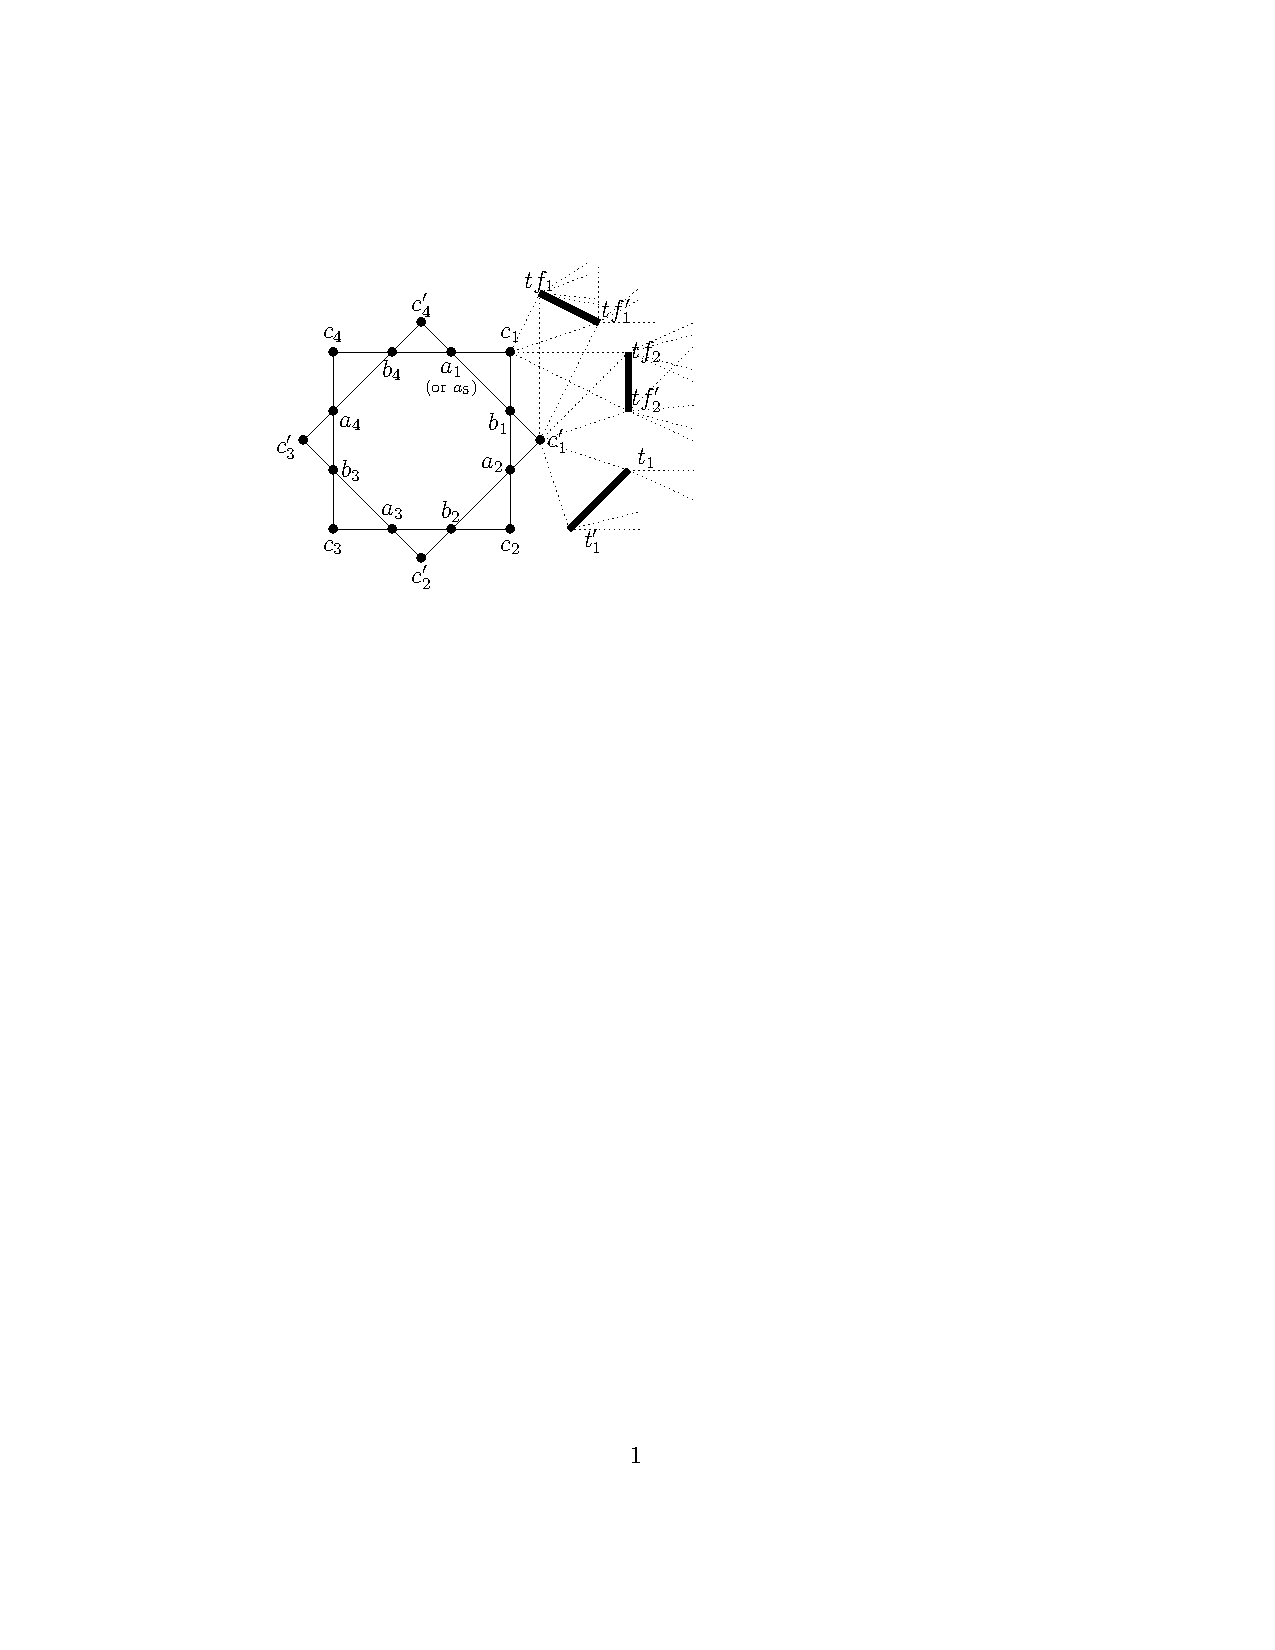
\includegraphics[trim = 120 500 300 120, clip, width=\linewidth]{figures/deDuplication/pccHardQuery.pdf}
			\end{figure}
		\end{column}

		\begin{column}{0.48\textwidth}
			\begin{itemize}
				\item Literal $x_1$ is part of four different clauses.
				\item $(a_i, b_i, c_i)$ capture truth assignment and $(b_i, c_i', a_{i+1})$ captures false assignment.
				\item Hyper-edges containing $tf_i, tf_i'$ and $t_1, t_1'$ capture truth setting for the clause $C = \{x_1, x_2, x_3\}$.
				
			\end{itemize}
		\end{column}
	\end{columns}	
	\begin{itemize}
		\item $t_1, t_1'$ ensure that atleast one of the literals is true. 
	\end{itemize}
\end{frame}

\begin{frame}{Goals}
	Computation complexity of PCC.
	\begin{itemize}
		\vspace{10pt}\item NP-Hard.
	\end{itemize}	 
	\vspace{10pt}Computation complexity in the presence of an oracle.
	\begin{itemize}
		\vspace{10pt}\item Hard for $o(|X|)$ queries.
	\end{itemize}

    \Huge{
    \begin{center}
    	Disappointing !!\\
    	\Frowny{} 
   	\end{center}
    }
\end{frame}

\begin{frame}{Circumventing the hardness?}
	Possible approach
	\begin{itemize}
		\item Design efficient approximation algorithms.		
	\end{itemize}
	
	\onslide<2->
	\vspace{30pt}Our approach
	\begin{itemize}
		\vspace{5pt}\item Limit the search space of clusterings $\mc F$.
		\vspace{5pt}\item Choose the best from a class of clusterings (or algorithms).
		\vspace{5pt}\item Useful tool for practitioners. 
	\end{itemize}
\end{frame}

\begin{frame}{Goals}
	\begin{itemize}
		\item Analyse computational and query complexity.
		\vspace{30pt}\item $\mc F = \{T_1, \ldots, T_s\}$ as a running example.\\
		\vspace{10pt}$T_i$ is a clustering tree.
	\end{itemize}
\end{frame}

\begin{frame}{Problem formulation: Attempt 1}
	Input: $X$\\
	Metric: $d$ over $X^2$.\\
	A class of clusterings: $\mc F$\\
	
	\vspace{20pt}Construct $G = (X, E)$, 
	
	\vspace{10pt}Output: 
	\vspace{-10pt}\begin{align*}
	  &\hat C = \argmin_{C \in \mc F} \enspace \text{correlation-loss}_{E}(C)
	\end{align*}
\end{frame}

\begin{frame}{Computationally easy}	
	Iterate over clusterings in $\mc F$		
	\begin{itemize}
		\vspace{10pt}\item Bottom-up traversal when $\mc F = $ trees.
	\end{itemize}
	\vspace{30pt}Choose the one with smallest loss.
	
\end{frame}


\begin{frame}{Restricted Correlation Clustering (RCC)}
	\begin{block}{Input}
		$(X, d)$, class of clusterings $\mc F$ and a $C^*$-oracle
	\end{block}
	
	\vspace{10pt}\begin{block}{Find}
		\vspace{-15pt}\begin{align*}
		  &\hat C = \argmin_{C \in \mc F} \enspace \text{correlation-loss}_{C^*}(C)
		\end{align*}	
	\end{block}
	
	\begin{block}{where}
		\vspace{-20pt}\begin{align*}
			d \text{ is }(\alpha, \beta)\text{-informative}&\\
			\text{correlation-loss}_{C^*}(C) &= \enspace  \mu \enspace \underset{(x, y) \sim P^+}{\mb P} \big[ C(x, y) = 0 ] \\
			&+\enspace (1-\mu) \enspace \underset{(x, y) \sim P^-}{\mb P} \big[ C(x, y) = 1] 
		\end{align*}
	\end{block}	
	$P^+$ is the uniform distribution over pairs where $C^*(x, y) = 1$
\end{frame}


\begin{frame}{Solution Strategy}
	\begin{block}{Algorithm}
		\begin{itemize}
			\vspace{10pt}\item Sample `enough' positive pairs.
			\vspace{10pt}\item Sample `enough' negative pairs.
			\vspace{10pt}\item Estimate correlation loss of each $C \in \mc F$.
			\vspace{10pt}\item Output clustering with minimum loss.
		\end{itemize}
	\end{block}
	
	\vspace{20pt}Uniform sampling doesn't work\\
	\vspace{10pt}Make use of informative metric $d$
\end{frame}

\begin{frame}{Goals}
	Computational complexity
	\begin{itemize}
		\vspace{10pt}\item Depends on the number of sampled points
		\vspace{10pt}\item Iterate over (or bottom-up traversal) over $\mc F$.
	\end{itemize}
	
	\vspace{30pt}Query complexity
	\begin{itemize}
		\vspace{10pt}\item Depends on the number of sampled points
	\end{itemize}
	
\end{frame}


\begin{frame}{Sampling negative pairs}
	
	\vspace{10pt}\textcolor{blue}{Basic Idea}\\
	Sample (with rejection) uniformly at random from $X^2$. 
	
	\vspace{20pt}\begin{block}{Results}
		The above procedure
		\begin{itemize}
			\item Samples a pair according to $P^-$.
			\item Makes $\frac{1}{1-\gamma}$ queries to the oracle in expectation. 
		\end{itemize}			
	\end{block}
	
	
\end{frame}

\begin{frame}{Sampling positive pairs}
	Recall the definition of $(\alpha, \beta)$-informative metric
	\vspace{-10pt}\begin{align*}
		&\underset{(x, y) \sim U^2}{\mb P}\enspace \big[d(x, y) > \lambda \enspace|\enspace C^*(x, y) = 1\big] \enspace \le \enspace \alpha \\
		&\underset{(x, y) \sim U^2}{\mb P}\enspace \big[C^*(x, y) = 1 \enspace|\enspace d(x, y) \le \lambda \big] \enspace \ge \enspace \beta
	\end{align*}

    
	\vspace{20pt}\textcolor{blue}{Basic Idea}\\
	Sample (with rejection) uniformly at random from $K = \{(x, y): d(x, y) \le \lambda\}$. 
\end{frame}

\begin{frame}{Sampling positive pairs}

	\begin{block}{Results}
		The above procedure
		\begin{itemize}
			\item Samples a pair according to distribution $T$ which approximates $P^+$.
			$$\Big|\underset{(x, y) \sim P^+}{\mb P}\enspace \big[ h(x, y) = 0 ] - \underset{(x, y) \sim T}{\mb P}\enspace \big[ h(x, y) = 0 ]\Big|  \enspace \le \enspace 2\alpha.$$ 
			The loss computed according to $T$ is similar to loss computed according to $P^+$ for any labeling function.
			\item Makes $\frac{1}{\beta}$ queries to the oracle in expectation. 
		\end{itemize}			
	\end{block}
	\vspace{20pt}\alert{$\Theta(n^2)$} time to construct set $K$.		
\end{frame}

\begin{frame}{Locality Sensitive Hashing}
	Use LSH to `approximately construct' set $K$.
	
	\vspace{20pt}Generic LSH scheme for input $X$:
	\begin{itemize}
		\vspace{10pt}\item Obtain $s$ different partitions of $X$.
		\vspace{10pt}\item Output $ B := \{P_1, \ldots, P_s\} = \{B_{ij} : 1\le i\le s, 1\le j \le |P_i|\}$
	\end{itemize}
	
	\vspace{20pt} 
	\begin{block}{Guarentee (informal)} 
		Most of the similar points ($d(x, y) \le \lambda$) are co-located in atleast one of the blocks $B_{ij}$ with high probability. 
	\end{block}
\end{frame}

\begin{frame}{Sampling for LSH-able metrics}
	\textcolor{blue}{Basic Idea}\\
	Sample (with two-step rejection) uniformly at random from the blocks $B$.
	\begin{itemize}
		\vspace{5pt}\item Reject with probability $= 1 - 1/$ \#blocks in which the pair occur together
		\vspace{5pt}\item Reject if the oracle says NO
	\end{itemize} 
\end{frame}

\begin{frame}{Sampling positive pairs for LSH-able metrics}
	\begin{block}{Results}
		The above procedure
		\begin{itemize}
			\item Samples a pair according to distribution $T$ which approximates $P^+$ (with high probability).
			\begin{align*}
  &\Big|\underset{(x, y) \sim P^+}{\mb P} \big[ C(x, y) = 0 ] -\underset{(x, y) \sim T}{\mb P} \big[ C(x, y) = 0 ] \Big| \le 2\alpha + \zeta  + \nu
  			\end{align*} 
			$\zeta$ depends on quality of the hashing and $\nu$ is a term that controls the probability. 
			\item Makes $O(\frac{1}{\beta})$ queries to the oracle in expectation. 
		\end{itemize}			
	\end{block}
\end{frame}

\begin{frame}{Recap}
	Procedure to sample $m_+$ positive pairs.\\

	\vspace{20pt}Procedure to sample $m_-$ negative pairs.\\
	\vspace{20pt}Estimate the loss from this sample.
\end{frame}

\begin{frame}{Main result}
	\begin{block}{Sample complexity}
		If the number of positive and negative samples   
		\vspace{-10pt}\begin{align*}
		  &m_-, m_+ \enspace \ge a\frac{\vcdim({\mc F}) + \log(\frac{3}{\delta})}{\epsilon^2} 
		\end{align*}
		then with probability atleast $1-\delta$, we have that $$L_{C^*}(\hat C) \enspace\le\enspace \min_{\mc C \in \mc F} L_{C^*}(C) + 3\alpha + \epsilon$$
	\end{block}
	
	\begin{itemize}
		\vspace{20pt}\item If we see enough samples then the loss of our clustering is close to the minimizer.\\
		\vspace{10pt} \item Independent of the size of the set $X$.
	\end{itemize}		
\end{frame}

\begin{frame}{Positive result: Queries}
	\begin{block}{Query complexity}
		With `high probability' the number of same-cluster queries $q$ made is  
		\vspace{-10pt}$$q \le (1+\nu)\bigg(\frac{m_-}{(1-\gamma)} + \frac{m_+}{\beta}\bigg)$$
	\end{block}
	\begin{itemize}
		\vspace{20pt} \item The number of wasted queries is small.
		\vspace{20pt} \item The number of queries depends only on the complexity of $\mc F$ and is independent of $|X|$.  
	\end{itemize}
\end{frame}

\begin{frame}{VC-Dimension of common classes}
	\begin{block}{Theorem}
		Let $\mc F = \{T_1, \ldots, T_s\}$ be a class of hierarchical clustering trees. Then 
		$$\vcdim({\mc F}) \le g(s)$$ where $g(s)$ is the smallest integer $n$ such that $\frac{\sqrt n!}{\lfloor \sqrt n/2 \rfloor! \enspace 2^{\lfloor \sqrt n/2 \rfloor}} \ge s $
	\end{block}
	
	\begin{itemize}
		\vspace{30pt}\item $\vcdim(T)$ is upper bounded by a constant.
		\vspace{10pt}\item Using standard theorems that would imply $\vcdim(\mc F) \le O(s)$
		\vspace{10pt}\item This result shows $o(\log^2 s)$ upper bound.
	\end{itemize}
\end{frame}

\begin{frame}{Key takeaways}
	For common classes of clusterings, 
	\begin{itemize}
		\vspace{30pt}\item ERM-based approach can solve the RCC problem efficiently. 
		\vspace{15pt}\item Query complexity of RCC depends on the complexity of $\mc F$.
	\end{itemize}
\end{frame}

\begin{frame}{Challenges in clustering}	
	\onslide<1>End of first part
	\vspace{10pt}\begin{block}{}
	\mynum{2} Under-specificity \alert{and} \\\vspace{10pt}\mynum{1} Computational complexity
	\end{block}
		
	\onslide<2>\vspace{35pt}Second part
	\vspace{10pt}\begin{block}{}
	\mynum{3} Noise-robustness \alert{and} \\\vspace{10pt}\mynum{1} Computational complexity
	\end{block}		
\end{frame}


\begin{frame}{Clustering definition: Revisit}
	Partition the input such that
	\begin{itemize}
		\vspace{10pt}\item Similar points share a cluster.
		\vspace{10pt}\item Dis-similar points are separated.
	\end{itemize}
	
	\vspace{30pt}Makes sense when the data is made of {\color{blue} cohesive subsets}.
\end{frame}

\begin{frame}{A more complex view}
	Besides nice structure, data also includes 
	\begin{itemize}
	  \item \alert{Unstructured} parts.
	\end{itemize}
	
	\vspace{30pt}
	Alternate definition of clustering that also allows for 
	\begin{itemize}
		\item A subset of ``{\color{blue}background noise}".
	\end{itemize}
	
\end{frame}

\begin{frame}{High-level problem definition}

	Input: $(X, d)$
	\vspace{20pt}

	Assuming the data consists of 
	\begin{itemize}
	\vspace{10pt}
	\item ``well clustered" subset $S$  
	\vspace{10pt}
	\item ``unstructured" complement $N= X \setminus S$
	\end{itemize}

	\vspace{30pt}
	{\color{blue} Output} a partition $C=(C_1, \ldots C_k)$ of $X$.
	\begin{itemize}
		\vspace{5pt}\item \emph{Induces} a good clustering of $S$. 
		\vspace{5pt}\item $C|_{S}$ recovers the structure.
	\end{itemize}

\end{frame}

\begin{frame}{Clustering in the presence of sparse noise}
	\begin{itemize}
		\item Joint work with Samira Samadi (Phd candidate at Georgia Tech) and Shai Ben-David.
		\vspace{20pt}\item In proceedings of \alert{ALT'16}. 
	\end{itemize}
\end{frame}

\begin{frame}{Definitions}

	Given $(X, d)$, a set $S \subseteq X$\\
	\vspace{0.5cm}A clustering $\mc C = \{S_1, \ldots, S_k\}$ of the set $\mc S$ induced by centers $s_1, \ldots, s_k$.

	\vspace{10pt}\begin{block}{$(\alpha, \eta)$-center proximity}
	\vspace{0.5cm} {\bf $\alpha$-center proximity}: For all $x \in S_i$ and $i\neq j$, $$\alpha d(x, s_i) < d(x, s_j)$$
	{\bf $\eta$-sparse noise}: For any ball $B$, 
	$$r(B)\leq \eta \thinspace r(\mc{C}) \implies |B\cap (\mc X\setminus \mc S)| < \frac{m(\mc C)}{2}$$
	\end{block}
\end{frame}


\begin{frame}{Sparse Noise}
    Any ball of small radius contains few points from $N$.
    \begin{figure}
	  \includegraphics[trim = 100 0 0 100, clip, width=\linewidth]{figures/clusteringNoise/2.pdf}
   \end{figure}
    	 
\end{frame}

\begin{frame}{Our Results}
 \alert{Positive results}
 
 \begin{itemize}
  	\item $\alpha > 4.6$ and noise is sparse\\ 
	
	
	\textcolor{blue}{We construct  in poly time a clustering tree that induces the original nice clustering}.
  	
	\begin{figure}
	  \includegraphics[trim = 50 150 50 200, clip, width=0.8\linewidth]{figures/clusteringNoise/hier.pdf}
	\end{figure}	  	
  \end{itemize}  
\end{frame}

\begin{frame}{Our Results}
\alert{Negative results}
  \begin{itemize}
  	\vspace{10pt}\item $\alpha < 5.8$ and noise is adversarial, or 
	\vspace{10pt}\item $\alpha < 4.4$ and noise is sparse
\end{itemize}

	 \vspace{30pt}\textcolor{red}{One cannot guarantee efficient recovery of the non-noise clustering}. 
\end{frame}


\begin{frame}{Clustering under $(\alpha, \eta)$-center proximity}
	\begin{block}{The algorithm}
	  Input: $(X, d)$ and a parameter $t$.\\
	  Output: A hierarchical clustering tree.\\
	  \vspace{20pt}Initialize every point in its own cluster.\\
	  \vspace{10pt}Go over all pairs of points $p, q$ in increasing order of distance.\\
	  \vspace{10pt}If $B := B(p, d(p, q))$ satisfies the \alert{sparse-distance condition}
	  \begin{itemize}
	  	\item Merge all clusters that intersect with $B$ into a single cluster
	  \end{itemize}
    \end{block}

\end{frame}


\begin{frame}{Sparse-distance condition}
    All clusters that intersect with $B$ should have a non-sparse intersection. 
	\begin{itemize}
	  \item $|B| \ge t$.
	  \item For any $X_i \in \mc C$, if $X_i \cap B \neq \emptyset$, then $X_i \subseteq B$ or $|B \cap X_i| \ge t/2$.
	\end{itemize}

   \begin{figure}
	  \includegraphics[trim = 100 0 0 100, clip, width=\linewidth]{figures/clusteringNoise/3.pdf}
   \end{figure}
\end{frame}

\begin{frame}{Sparse-distance condition failure}   
   \begin{figure}
	  \includegraphics[trim = 100 0 0 100, clip, width=\linewidth]{figures/clusteringNoise/4.pdf}
   \end{figure}
\end{frame}

\begin{frame}{Positive results}
	\begin{itemize}
		\item \textit{Captures} all clusterings which satisfy $(2+\sqrt{7}, 1)$-center proximity.
	
		\vspace{30pt}\item Runs in time $O(|X|^3)$.
	
		\vspace{30pt}\item Results \alert{don't} depend on any \alert{upper bound} on $|N|$.
	\end{itemize}
\end{frame}

\begin{frame}{Lower bound}
	If $\alpha < 3 + \sqrt{2}$ and noise is sparse
	\begin{itemize}
		\item No clustering tree can capture all nice solutions.
	\end{itemize}
	
	\vspace{20pt}\begin{figure}[!t]
	  \begin{center}
	    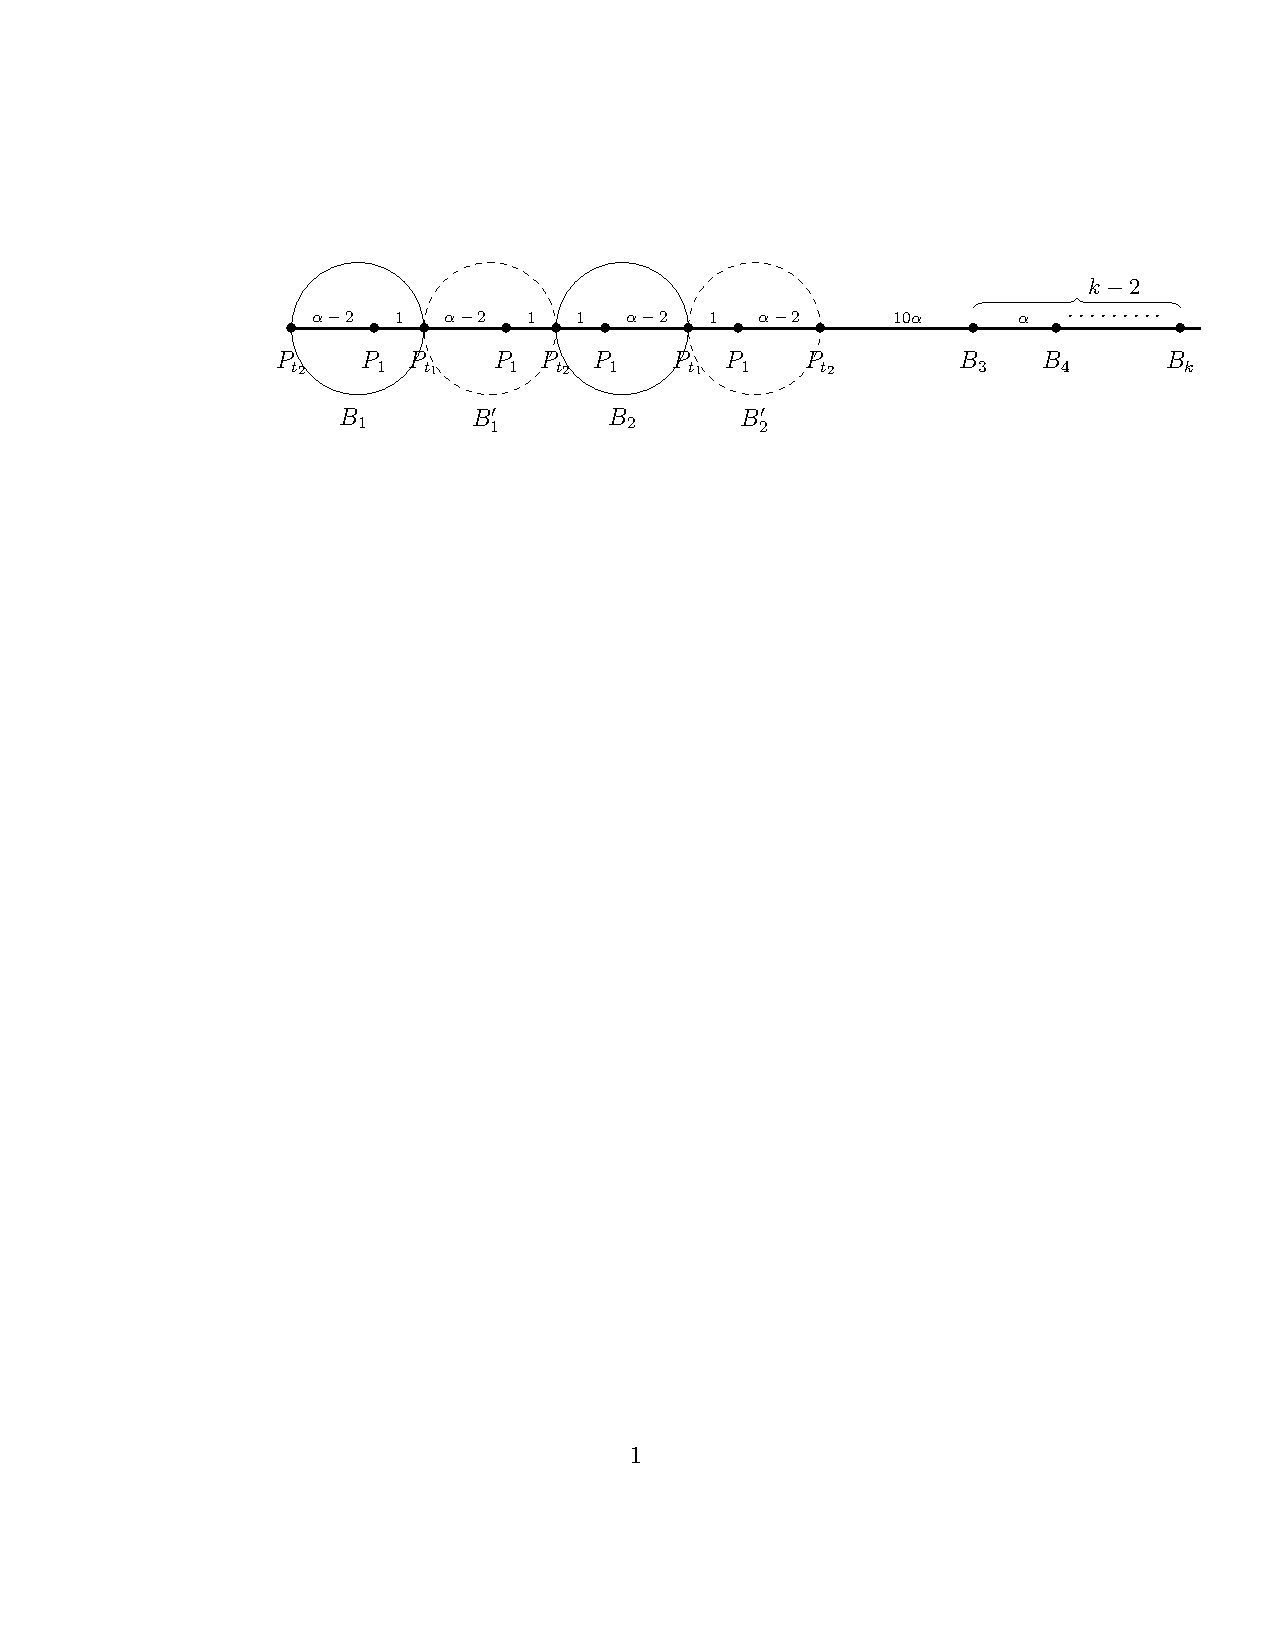
\includegraphics[trim={47mm 205mm 12mm 44mm},clip,width=\textwidth]{figures/clusteringNoise/lbdFig2.pdf}
	  \end{center}
	\end{figure}
	\vspace{20pt}Same ideas can be extended to a list output.\\
	\begin{itemize}
		\item Any list should have size $> 2^{k/2}$
	\end{itemize}
\end{frame}

\begin{frame}{Possible justification of sparse noise}
    \begin{itemize}
	  \item Data $\mc S$ has nice structure.
	  \vspace{20pt}\item Noise $\mc N$ is added by a non-concentrated distribution.
	  \vspace{30pt}\item $\mc X = \mc S \cup \mc N$ satisfies the structureless noise definition with high probability.
    \end{itemize}
\end{frame}

\begin{frame}{Key Takeaways}
	\begin{itemize}
		\item Notion of sparse noise to handle background noise.
		\vspace{25pt}\item Efficient hierarchical algorithm that captures {\color{blue}all nice} solutions.
		\vspace{25pt}\item Positive result {\color{blue}independent} of the number of noisy points.
	\end{itemize}
\end{frame}

\begin{frame}{Noise-robust clustering objectives}
	\begin{itemize}
		\item Joint work with Yaoliang Yu and Shai Ben-David.
		\vspace{25pt}\item Available on \alert{arxiv'18}. 
		\vspace{20pt}\item Under submission. 
	\end{itemize}
\end{frame}

\begin{frame}{Problem definition}
	Input: $(X, d)$
	\vspace{20pt}

	Assuming $X = S \cup N$

	\vspace{20pt}
	{\color{red} Output} a partition $C= \{C_1, \ldots C_k\}$
	\begin{itemize}
		\vspace{5pt}\item \emph{Induces} a good clustering of $S$. 
	\end{itemize}
	
	\vspace{20pt}Algorithms based on {\color{blue} optimizing} a {\color{blue} suitable clustering objective} function.
\end{frame}

\begin{frame}{Simple observations}
	$k$-means or $k$-median type objectives can \alert{break} with one outlier.
	\begin{itemize}
		\item $$\sum_{i =1}^k\enspace\sum_{x \in C_i} \|x - \mu_i\|^2$$		
		\vspace{10pt}\item Place outlier at `infinity'.
		\vspace{10pt}\item Allowing $p$ extra clusters doesn't work for $p+1$ outliers. 
	\end{itemize}
\end{frame}

\begin{frame}{Robustifing clustering objectives}
	$\lambda$-regularized paradigm.
	\begin{itemize}
		\vspace{5pt}\item $$\sum_{i =1}^k\enspace\sum_{x \in C_i} \|x - \mu_i\|^2 \enspace+\enspace \textcolor{red}{\lambda |C_{k+1}|}$$
		\vspace{20pt}\item Discard points into a garbage cluster.
	\end{itemize}
	
	\vspace{20pt}\textcolor{blue}{Can regularization help with noise-robustness?}
\end{frame}

\begin{frame}{Sidenote: Properties of the regularized objective}	
	For all $\lambda$
	\begin{itemize}
		\item For all clustering instances 
		\begin{itemize}
			\vspace{10pt}\item Easy for $\lambda \le \frac{m(X)}{2}$.
			\vspace{10pt}\item Reduces to classical $k$-means for $\lambda \ge \frac{M(X)}{2}$.			
		\end{itemize}
		\vspace{20pt}\item There exists instance which are NP-Hard for $\textcolor{blue}{k \ge 1}$ if $$\frac{m(X)}{2} < \lambda$$
	\end{itemize}
\end{frame}

\begin{frame}{Tackling computational hardness}
	$$\text{Original objective} \longrightarrow \text{Convex relaxation}$$
	
	\vspace{20pt}Tightness under the {\color{blue}stochastic ball assumption}.
	\begin{itemize}
		\vspace{10pt}\item $k$ unit balls separated by $\delta$
		\vspace{10pt}\item Generated by isotropic distribution. 
	\end{itemize}	
\end{frame}

\begin{frame}{Previous work under the stochastic ball model}
	\begin{table}
		\centering
		\label{table:stochasticBall}
		\setlength{\tabcolsep}{0.7em} 
		{\renewcommand{\arraystretch}{1.5}%
		\begin{tabular}{llc}
		\\
		 & Separation condition & Reference\\
		 \hline
		$k$-median LP & $\delta > 3.75$ & \alert{[Nellore et. al' 15]}\\
		 & $\delta > 2$ & \alert{[Awasthi et. al'15]}\\
		\hline
		$k$-means LP & $\delta > 4$ & \alert{[Awasthi et. al'15]}\\
		\hline
		$k$-means SDP & $\delta > 2\sqrt2 (1 + \frac{1}{\sqrt d})$ & \alert{[Awasthi et. al'15]}\\
		 & $\delta > 2 + \frac{k^2}{d}cond(\gamma)$ & \alert{[Iguchi et. al'15]}\\
		 & $\delta > 2 + \frac{k^2}{d}$ & \alert{[Iguchi et. al'17]}\\

		\label{table:alphacenter}
		\end{tabular}
		}
	\end{table}
\end{frame}

\begin{frame}{Recall: Framework}
	Input $X =  S \cup N$ where
	\begin{itemize}
		\vspace{10pt}\item $S = \cup_{i=1}^k B_i$
		\vspace{10pt}\item $S$ is generated by an isotropic distribution. 
		\vspace{10pt}\item $r(B_i) \le 1$ and $\|\mu_i - \mu_j\| > \delta$.
	\end{itemize}
	
	\vspace{20pt}Design an efficient algorithm  $\mc A$ that induces the target clustering. 
\end{frame}

\begin{frame}{SDP-based relaxation}
	Equivalence of the regularized objective 
	$$\sum_{i =1}^k\enspace\sum_{x \in C_i} \|x - \mu_i\|^2 \enspace+\enspace \lambda |C_{k+1}|$$ to the following.
	
	$$	
	\text{0-1 SDP}
	\begin{cases}
		\min_{Z, y} \enspace &\tr(DZ) + \lambda \langle \mb 1, y\rangle\\
		\text{s.t. } \enspace &\tr(Z) = k\\
		& Z\cdot \mb 1 + y = \mb 1\\	
		&Z\ge 0, Z^2 = Z, Z^T = Z \\
		& y \in \{0, 1\}^n
	\end{cases}	
	$$
\end{frame}

\begin{frame}{SDP-based relaxation}
	Relaxation of the regularized objective gives
	$$	
	\text{Regularized SDP}
	\begin{cases}
		\min_{Z, y} \enspace &\tr(DZ) + \lambda \langle \mb 1, y\rangle\\
        \text{s.t. } \enspace &\tr(Z) = k\\
		& \Big(\frac{Z+Z^T}{2}\Big)\cdot \mb 1 + y = \mb 1\\		
		&Z \ge 0, y \ge 0\\
		& Z \succeq 0
	\end{cases}
	$$
\end{frame}

\begin{frame}{Main result}
	%Mildness properties of $N$.
	%\begin{itemize}
	%	\item {\color{blue}Far} - $\|n_2 - x\| \ge \nu \ge \sqrt{(\delta-1)^2+1}$.
	%	\begin{center}OR\end{center}
	%	\item {\color{blue}Small margin} - $| \|n_1-\mu_i\|^2 - \|n_1-\mu_j\|^2| \ge \alpha$
	%\end{itemize}
	\begin{theorem}
	 If  
	\begin{itemize}
	  \item $\delta > 2 + \sqrt{ O(\zeta) + \frac{k}{d}}$ 
	  %\item $\alpha \ge O(\zeta)+ \frac{k}{d}$ 
	  %\item $\frac{|N_2|}{n} \le \frac{\delta^2-2\delta-O(\zeta)}{\lambda}$	  
	\end{itemize}
	and the noise satisfies certain mildness conditions (relative to the size and distance to $S$) then the regularized $k$-means SDP outputs the clustering $C$ such that
	$$C|_{S} = \{B_1, \ldots, B_k\}$$
	%Let $n = \min_i |B_i|$ and $\zeta = \frac{|N_1|}{n}$. 
	\end{theorem}
	
	\vspace{20pt}{\color{blue}Corollary}\\
	For the noiseless case, the $k$-means SDP finds the desired clustering for $$\delta > 2 + \sqrt{\frac{k}{d}}$$
\end{frame}

\begin{frame}{Key Takeaways}
	\begin{itemize}
		\item Considered regularized $k$-means objective.
		\vspace{20pt}\item Regularization can help with noise robustness especially noisy points.
	\end{itemize}
\end{frame}

\begin{frame}{Thesis takeaways}
	\begin{itemize}
		\item Three challenges faced during design of clustering algorithms.
		\vspace{20pt}\item Semi-supervision can help with under-specificity and computational hardness.
		\vspace{20pt}\item Algorithmic paradigms for dealing with noise-robustness issues.
	\end{itemize}
\end{frame}
\begin{frame}
    \Huge{\centerline{Thank You!}}
\end{frame}

\begin{frame}{CC framework: Missing pieces}
	Two options
	\begin{enumerate}
		\item Adding information ``stored" in the the edges $E$
		\vspace{10pt}\item Adding human supervision
	\end{enumerate}
	
	\vspace{20pt}Proved that
	\begin{enumerate}
		\item alone doesn't help (just proved)
		\vspace{10pt}\item alone doesn't help (proved by others)
	\end{enumerate}
	
	\vspace{20pt}How about \mynum{1} and \mynum{2}?
\end{frame}

%----------------------------------------
%        Figure Samples
%----------------------------------------

% All of the following is optional and typically not needed. 
\appendix
\section<presentation>*{\appendixname}
\subsection<presentation>*{For Further Reading}



\end{document}



